\documentclass[10pt]{article}

\usepackage[margin=0.75in]{geometry}
\usepackage{amsmath,amsthm,amssymb}
\usepackage{xcolor}
\usepackage{cancel}
\usepackage{graphicx}
\usepackage{changepage}
\usepackage{circuitikz}
\usepackage{pgfplots}
\usepackage{physics}
\usepackage{hyperref}
\usepackage{siunitx}
\usepackage{fontspec}
\usepackage{relsize}
\usepackage{subfig}
\usepackage{minted}
\usepackage{todonotes}
\usepackage{adjustbox}
\usepackage{pdfpages}
\usepackage{multicol, multirow, booktabs}
\usepackage[breakable]{tcolorbox}
\usepackage[inline]{enumitem}

\theoremstyle{definition}
\newtheorem{problem}{Problem}
\newtheorem{soln}{Solution}

\pgfplotsset{compat=newest}
\usetikzlibrary{lindenmayersystems}
\usetikzlibrary{arrows}
\usetikzlibrary{calc}
\usetikzlibrary{positioning, fit}
\usetikzlibrary{3d, perspective}

\definecolor{incolor}{HTML}{303F9F}
\definecolor{outcolor}{HTML}{D84315}
\definecolor{cellborder}{HTML}{CFCFCF}
\definecolor{cellbackground}{HTML}{F7F7F7}
\newcommand{\ui}{\hat{i}}
\newcommand{\uj}{\hat{j}}
\newcommand{\uk}{\hat{k}}
\newcommand{\ux}{\hat{x}}
\newcommand{\uy}{\hat{y}}
\newcommand{\uz}{\hat{z}}
\newcommand{\primed}[1]{#1^\prime}
\pgfdeclarelayer{background}  
\pgfsetlayers{background,main}
\AtBeginDocument{\RenewCommandCopy\qty\SI}
\definecolor{LightGray}{gray}{0.9}

\makeatletter
\newcommand{\boxspacing}{\kern\kvtcb@left@rule\kern\kvtcb@boxsep}
\makeatother
\newcommand{\prompt}[4]{
    \ttfamily\llap{{\color{#2}[#3]:\hspace{3pt}#4}}\vspace{-\baselineskip}
}

\newcommand{\thevenin}[2]{
  \begin{center}
    \begin{circuitikz} \draw
      (0,0) -- (2,0) to[battery1, l_=$V_{Th}\eq#1$] (2,2) 
      to[resistor, l_=$R_{Th}\eq#2$] (0,2)
      ;
      \draw [o-] (-.07,2.079);
      \draw [o-] (-.07,0.079);
    \end{circuitikz}
  \end{center}
}

\newcommand{\norton}[2]{
  \begin{center}
    \begin{circuitikz} \draw
      (0,0) -- (3,0) to[american current source, l_=$I_{N}\eq#1$] (3,2) -- (0,2) (2,0)
      to[resistor, l=$R_{N}\eq#2$] (2,2)
      ;
      \draw [o-] (-.07,2.079);
      \draw [o-] (-.07,0.079);
    \end{circuitikz}
  \end{center}
}


\newcommand{\highlight}[1]{\colorbox{yellow}{$\displaystyle #1$}}

\newcommand{\ti}[1]{\widetilde{#1}}

\newfontface{\Kaufmann}{Kaufmann}
\DeclareTextFontCommand{\kf}{\Kaufmann}
\newcommand{\scriptr}{\fontsize{12pt}{12pt}\kf{r}}

\newfontface{\KaufmannB}{Kaufmann Bd BT}
\DeclareTextFontCommand{\kfb}{\KaufmannB}
\newcommand{\bscriptr}{\fontsize{12pt}{12pt}\kfb{r}}

\newcommand{\bv}[1]{\mathbf{#1}}

\title{Physics 4050H: Project 1}
\author{Jeremy Favro (0805980), Melody Berhane () \\\emph{Department of Physics \& Astronomy}\\ Trent University, Peterborough, ON, Canada}
\date{\today}

\begin{document}
\maketitle
\listoftodos

\begin{abstract}
  We successfully automated PHYS-2250H's lab 4 on operational amplifiers through microcontroller operated
  wave generation and input element switching, however due to time constraints did not automate data collection.
  The automation functions well with issues only in the imperfect connections of the breadboard sometimes causing
  disconnects when disturbed.
\end{abstract}
\section{Introduction}
The goal of this project was to take a lab from PHYS-2250H (Electronics) and improve upon/automate the content of that lab. We opted to
automate lab 4 which involved constructing different configurations of operational amplifiers and verifying that the theoretical equations
derived in lecture corresponded to the real-world behaviour of the device. Lab 4 specifically looked at varying the input resistance of an
inverting amplifier and looked at a single configuration of differentiating amplifier. Our initial concept for automation was to go the most direct route
and use a microcontroller to control a switch which would allow selecting different components as in the case of both the inverting and differentiating amplifiers
the only component which is varied between measurements is the element lying between the signal source and inverting input of the amplifier. We additionally
sought to eliminate as many components external to those which sit directly on a breadboard and so created a (single) function generator to replace the one used in the original lab.
\newpage
\section{High Level Overview}
\begin{figure*}[h]
  \centering
  \begin{circuitikz}[
      long/.style={circuitikz/bipoles/twoport/height=1.5}
    ]
    \draw[] (0,0) to[twoport, t=328P, name=gen328, long] ++ (2,0)
    (gen328.e) ++(1.7,0) node[above]{SPI Control}
    (gen328.e) -- ++(2.2,0) to[dac, name=mcp, anchor=west, l=MCP4822] ++(2,0)
    (mcp.e) -- ++(0,0) to[amp, name=efa, t={E-F}] ++(2,0)
    (efa.e) -- ++(0.5,0) to[twoport, t=Switch, name=sw, long, style={circuitikz/bipoles/twoport/width=1.25}] ++(3,0)
    (sw.s) -- ++(0,0) to[twoport, t=328P, name=sw328, long] ++ (0,-2)
    (sw.e) to[resistor, l={Resistor Array}, name=rarr] ++(3,0)
    (rarr.e) -- ++(1,0) node[op amp, scale=0.75, anchor=-](fa){}
    (fa.-) -- ++(0,1) coordinate(R) to[resistor, l=$R_f$]  (R -| fa.out) -- (fa.out) -- ++(.5, 0) node[right]{$V_o$}
    ;
    \begin{pgfonlayer}{background}
      \draw
      node[fit={($(gen328.north)+(0,.5)$)
            ($(gen328.south)+(0,-.5)$)
            ($(gen328.west)+(0,-.5)$)
            ($(efa.east)+(0,.5)$)
          }, draw, fill=blue, opacity=0.2, dashed, label={Stage 1 - Wave Generator}, inner sep=10pt]{};
      \draw
      node[fit={($(sw.north)+(0,.5)$)
            ($(sw328.south)+(0,-.5)$)
            ($(sw328.west)+(0,-.5)$)
            ($(fa.out)+(0,.5)$)
          }, draw, fill=green, opacity=0.2, dashed, label={Stage 2 - Amplifier Control}, inner sep=10pt]{};
    \end{pgfonlayer}
  \end{circuitikz}
  \caption{Block Diagram of the Device. Note that the component labeled E-F is an emitter-follower/voltage follower op-amp}
\end{figure*}
The automation consists of two main stages, one which generates a fixed frequency and peak-to-peak voltage input and one
which controls which element is connected to the inverting input of the amplifier. There is technically a third stage which
provides power to the devices in the other two but it is a basic three component circuit comprised of a $\qty{5}{\volt}$ regulator and two
filter capacitors and is therefore left off of diagrams from hereon.
\subsection{Wave Generator}
The input signal generator uses a single ATMmega328P \cite{microchip:ATmega328P} (hereon referred to as a 328P) microcontroller connected through SPI
to an MCP4822\cite{microchip:MCP4822} digital-to-analog converter (DAC from hereon). The output of the DAC is passed
through a low-pass reconstruction filter, then to a emitter-follower/voltage-follower op-amp to stabilize the signal and then forwarded to
the second stage of the device.
\subsection{Amplifier Control}
This section of the device uses another 328P to control a 4 input/output switch where each input is connected
to the output of the first stage (the sine wave). Each output is connected then to a single resistor each
of which are in turn connected to the inverting input of an op-amp wired in an inverting configuration. The 328P
switches between each of these resistors every two seconds.
\section{Detailed Methods}
\subsection{Wave Generator}
The 328P runs the code seen in \ref{fgcode}. The ``algorithm'' used in the code is known as a phase accumulator.
A phase accumulator is convenient as it allows easy control of the frequency of the output wave desired frequency and
the number of samples in the lookup table.
At the beginning of the program we calculate a period over which the phase accumulator operates
and populate a lookup table with precalculated values of our desired output wave, sin in this case.
Then, for every iteration of the loop, we first check if sufficient time has passed to update the output of the DAC.
If not, we continue the loop. If sufficient time has passed
we first write out the value in our lookup table which corresponds to the current ``phase value''. We
then increment the phase modulo the size of our table so that it will wrap around to the beginning
when we reach the end of the table, then increment the next update time by our precalculated period.
Writing a value to the DAC involves, for the MCP4822, sending a 16-bit integer via SPI.
The contents of this integer, are, ordered from most to least significant bits,
4 command bits whose meanings are shown in \ref{fgcode} for our specific case and explained more generally
in the datasheet \cite{microchip:MCP4822}, then the 12-bit value to be written to the output of the DAC. Dependent
on command bits, this value may be a fraction of either 4096 (twice the internal voltage reference of the MCP4822)
or 2048. As our application requires a $1\unit{\volt}$ peak-to-peak wave, we opted for the latter. The 12-bit value
is then represented at the output of the DAC as the given fraction of the internal voltage reference. As
it becomes difficult to write with sufficient speed to produce a high-fidelity wave directly from the DAC
when high-frequencies are desired we only operate with 16 possible states for the output of the DAC. Because
we desire a smooth wave for the input of the op-amp we need to feed the stepped output that this
low sample count results in through a suitable reconstruction filter. Here this will be a filter which rejects
the sudden changes of the stepped wave and makes them more gradual, e.g. a low-pass filter. The output
of the DAC is already fed through a $\qty{1}{\kilo\ohm}$ current limiting resistor so we opted to include
a $\qty{1}{\micro\farad}$ capacitor to ground in parallel with this output resistor, giving a time constant of
$\qty{1}{\milli\second}$ which, though not exactly the same as our sampling frequency, gives a sufficiently smoothed wave
and was chosen based on on-hand components. For the final step of this first stage of the whole device we feed the signal
through an emitter-follower amplifier to pass the loading created by the second stage
from the DAC to an op-amp which fixes the output voltage at the voltage generated by the DAC.
\subsection{Amplifier Control}
The amplifier control circuit is much simpler than the frequency generator and is comprised
of a single 328P running the code found in \ref{mcode} which is dedicated to switching four of its digital output pins between high and
low in sequence. These pins are connected to the control pins of an SN74HC4066N \cite{TI:sn74hc4066} whose input pins are chained
together and connected to the output of stage 1 (the emitter-follower output). Each output pin of the switch
is then connected to a $\qty{220}{\ohm},\qty{1}{\kilo\ohm}, \qty{3.6}{\kilo\ohm}, \qty{9.1}{\kilo\ohm}$ resistor, each of which are
in turn connected to the inverting input of our final op-amp. We then have the inverting input connected to the output
through a $\qty{10}{\kilo\ohm}$ resistor (and the non-inverting input connected to ground) to create a variable
inverting amplifier.
\section{Conclusion}
Generally the project was a success insofar as automation is concerned.
\subsection{Areas for Improvement}
\subsubsection{Automated Measurement}
The 328P is capable of analog reads from $0-\qty{5}{\volt}$. The amplifier stage of the device outputs above this range but
could be divided down with a voltage divider to allow automatic measurement of both the input and output signals of the inverting amplifier.
Depending on desired functionality these signals could be sent over USB (though this would require a suitable interface if the 328P was to remain
in the breadboard rather than the Arduino) or to a breadboard mounted display to eliminate the need for external measurement devices.
\subsubsection{Current Element Display \& Manual Element Switching}
Currently the arduino controlling the switch operates on a two second timer where each input element is on for two seconds before the device switches to the next.
As an extra feature, it would not be difficult to add a button or other input device which would allow a user to decide when they want to switch between
different input elements. In addition to this it may be nice to have a display controlled by the switching 328P to indicate which input element is currently selected.
This could be a display element such as an LCD or just LEDs tied to the control inputs of the switch to indicate which is selected, though an LCD
would be more clear.
\subsubsection{Differentiating op-amp}
The original version of the lab automated here included a fifth input element, a $\qty{0.1}{\micro\farad}$ capacitor in the same location as the resistors
to create a differentiating amplifier. Adding this alongside the 4 resistors would require either a different switch with more I/O pins or a second switch.
One of the existing resistors could also easily be switched out for a capacitor, probably either of the two middle valued ones as the upper and lower ones
exhibit more interesting properties with $\qty{220}{\kilo\ohm}$ having a clipped waveform due to over driving the amplifier and $\qty{9.1}{\kilo\ohm}$ having a
gain of near $1$ and therefore acting nearly as an inverter alone.
\section{References}
\bibliographystyle{plain}
\bibliography{sources}{}
\section{Appendix}
\subsection{Switch Control Code} \label{mcode}
\inputminted[
  frame=lines,
  framesep=2mm,
  baselinestretch=1.2,
  bgcolor=LightGray,
  fontsize=\footnotesize,
  linenos,
  breaklines
]{cpp}{./measurement/measurement.ino}
\subsection{Frequency Generator Code} \label{fgcode}
\inputminted[
  frame=lines,
  framesep=2mm,
  baselinestretch=1.2,
  bgcolor=LightGray,
  fontsize=\footnotesize,
  linenos,
  breaklines
]{cpp}{./sinegen/sinegen.ino}
\subsection{Full Schematic}
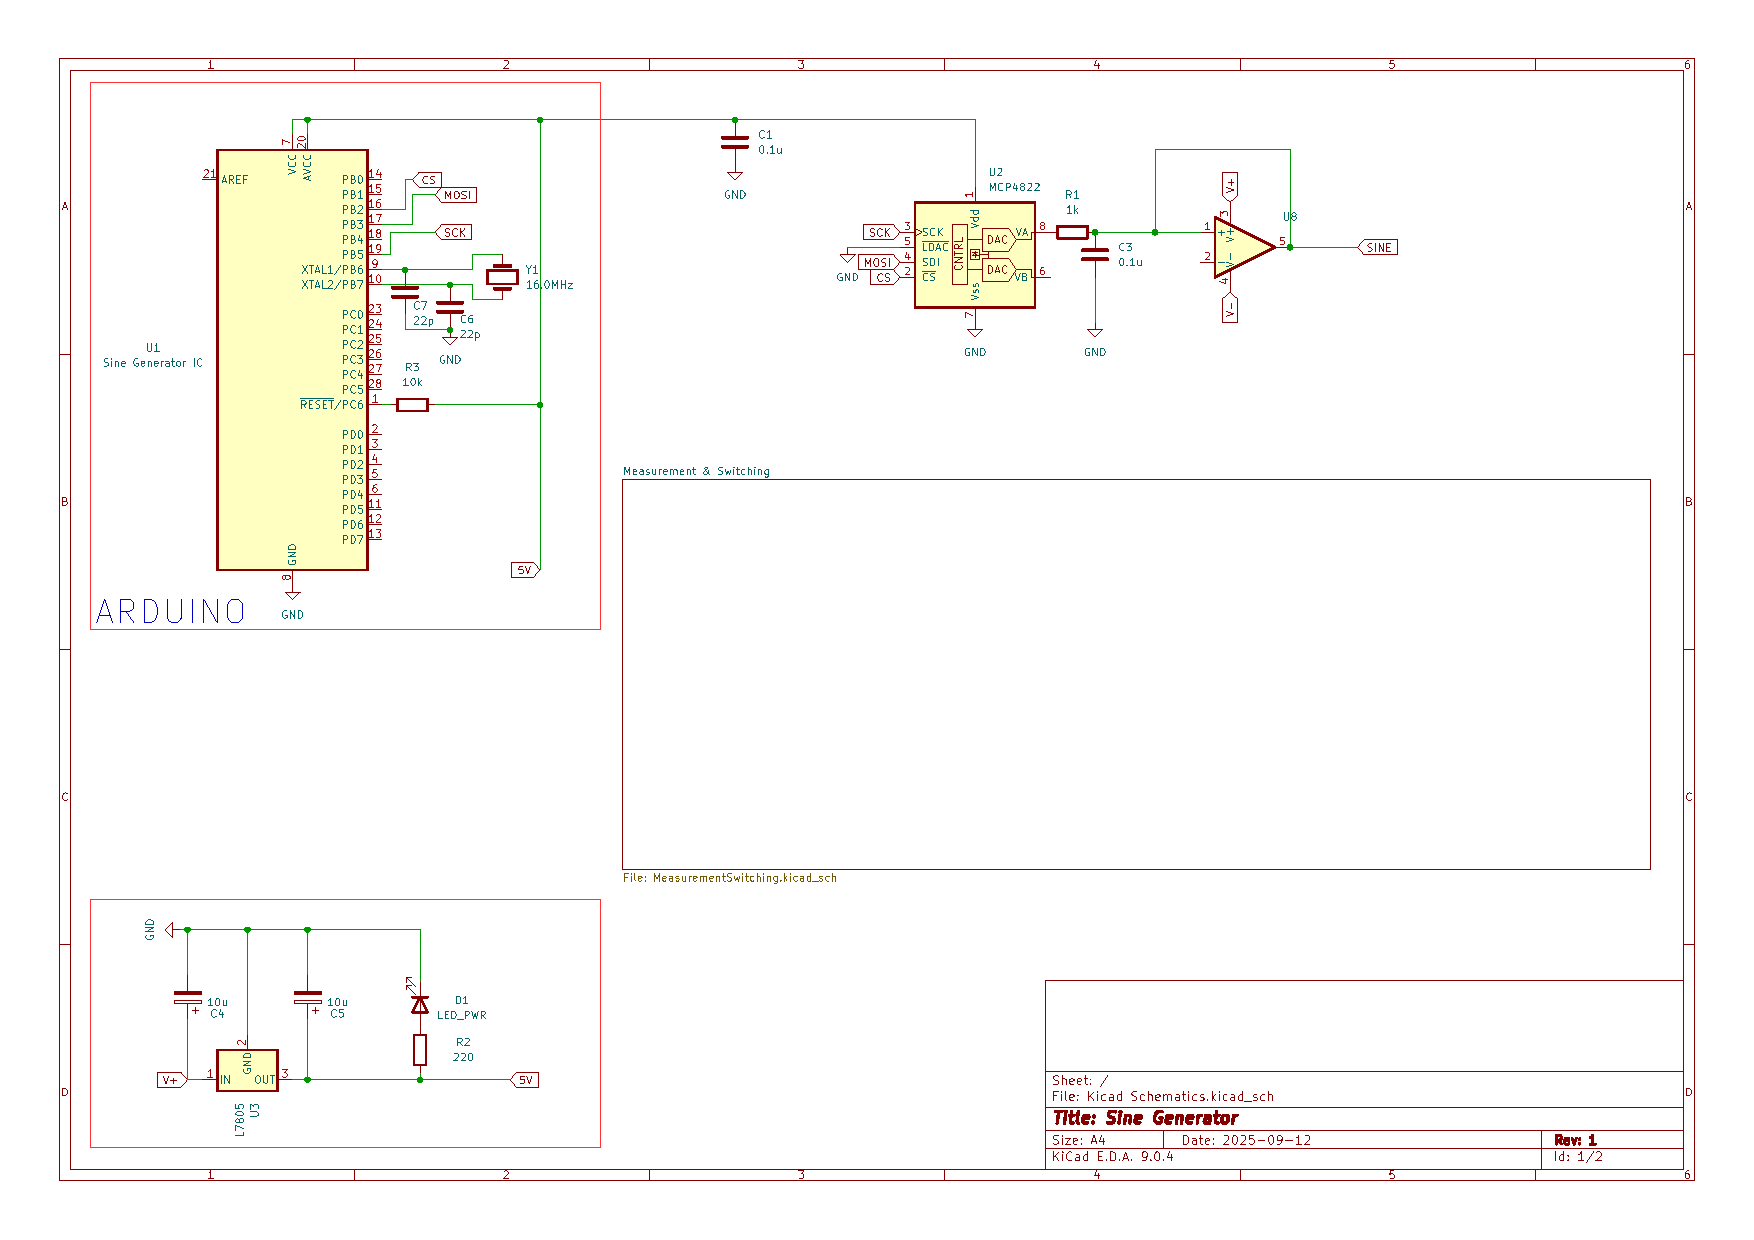
\includepdf[pages={1-2}, landscape]{./Kicad Schematics/Kicad Schematics.pdf}
\end{document}